\documentclass[11pt]{report}

% --- Language ---
\usepackage[french]{babel}
\usepackage[T1]{fontenc}
\usepackage[utf8]{inputenc}

% --- Figures ---

% Images
\usepackage{graphicx}
\graphicspath{{img/}}


% --- Code ---
\usepackage{minted}


% --- Layout ---
% Cover
\usepackage{titling}

% Page
\usepackage[a4paper, left=2.5cm, right=2.5cm, top=2.5cm, bottom=2.5cm]{geometry}
\usepackage{lscape}

% Font
\usepackage{libertine}

% Spacing
\renewcommand{\baselinestretch}{1.25}

% Sectioning
\renewcommand{\thesubsection}{\thesection.\alph{subsection}}

% Colors
\usepackage{xcolor}

% --- Drafting ---
\usepackage[section]{easy-todo}

\begin{document}

\begin{titlepage}
	\centering
	
\includegraphics[scale=0.8]{logo}\\
	\vspace{5cm}
	{\Huge{ \bf{VISA}}}\\
	\vspace{0.5cm}
   	{\Huge{\bf {TP 9}}}\\
	\vspace{2cm}
   	{\huge{Logique floue}}\\
	\vspace{3cm}
   	{\large{Quentin Brault}}
\end{titlepage}

\listoftodos
%\lstset{
%	language=C++,
%	frame=single,
%	keywordstyle=\color{blue},
%	stringstyle=\color{red},
%	commentstyle=\color{OliveGreen},
%	morecomment=[l][\color{magenta}]{\#}
%}
\section*{1. Fonctions d'appartenance}

\subsection*{a) Ensembles flous}
Chaque fonction d'appartenance est décrite par une fonction qui prend une valeur en entrée et retourne un résultat entre 0 et 1 correspondant à cette valeur.\\
Dans notre cas, la valeur en entrée peut être n'importe quel nombre entre 0 et 40, ce qui correspond à la température en °C, et il y a 3 fonctions d'appartenance (température basse, moyenne et élevée).\\
Ces trois fonctions d'appartenance prennent la forme d'un trapézoïde, donc j'ai d'abord créé une fonction trapézoïde générique qui sera réutilisée par chacune des fonctions d'appartenance.\\
a, b, c et d représentent la position sur l'axe des abscisses des 4 coins du trapézoïde. Sur l'axe des ordonées, les coins associés à a et d ont une valeur de 0 et les points associés à b et c ont une valeur de 1.
\begin{minted}{python}
def fuzzy_trapezoid(a, b, c, d, x):
    if a < x < b:
        return (x - a) / (b - a)
    if b <= x <= c:
        return 1
    if c < x < d:
        return (d - x) / (d - c)
    return 0
\end{minted}

On peut donc maintenant définir nos fonctions d'appartenance en se basant sur le graphique donné..
\begin{minted}{python}
def low_temp(temperature):
    return fuzzy_trapezoid(0, 0, 10, 20, temperature)

def medium_temp(temperature):
    return fuzzy_trapezoid(10, 20, 20, 30, temperature)

def high_temp(temperature):
    return fuzzy_trapezoid(20, 30, 40, 40, temperature)
\end{minted}

Pour vérifier notre ensemble, on peut appeler ces fonctions en itérant sur les abscisses et dessiner le graphe correspondant.
\begin{center}
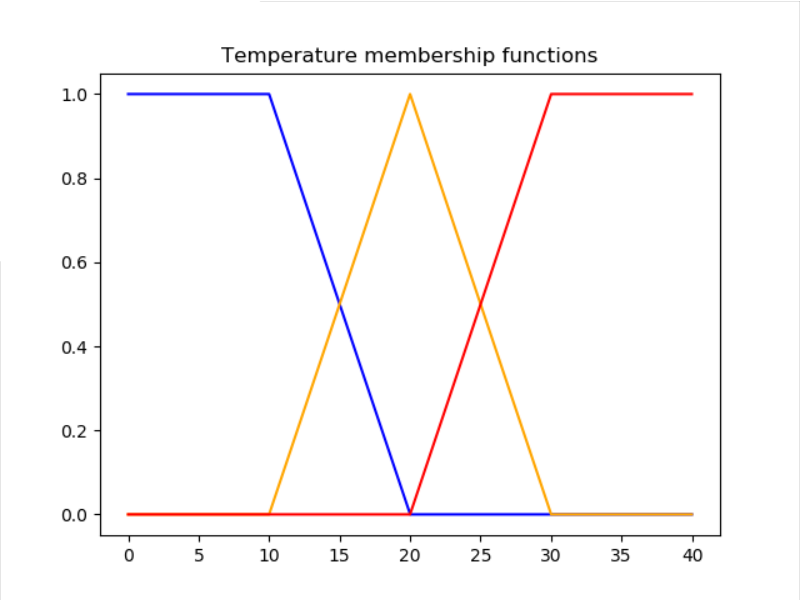
\includegraphics[width=300px]{membership_functions}
\end{center}

\subsection*{b) Degrés d'appartenance}
J'ai créé une fonction our récupérer les degrés de chaque fonction d'appartenance en une valeur donnée.
\begin{minted}{python}
def fuzzy_grades(membership_functions, value):
    return [membership_function(value) for membership_function in membership_functions]
\end{minted}

On peut donc appeler cette fonction avec nos fonctions d'appartenances et la valeur 16 pour trouver les degrés d'appartenance de chaque fonction à 16°C.
\begin{minted}{python}
membership_functions = [low_temp, medium_temp, high_temp]
print(fuzzy_grades(membership_functions, 16))
>> [0.4, 0.6, 0]
\end{minted}

\subsection*{c) Température basse ou moyenne}

J'ai commencé par créer une fonction qui retourne le OU de deux valeurs provenant d'une fonction floue. J'ai également ajouté les fonctions logiques NOT et AND.
\begin{minted}{python}
def fuzzy_not(grade):
    return 1 - grade

def fuzzy_or(grade1, grade2):
    return max(grade1, grade2)

def fuzzy_and(grade1, grade2):
    return min(grade1, grade2)
\end{minted}
Le NOT correspond à 1 moins la valeur, car nos valeurs sont entre 0 et 1.
Le OR correspond au max des deux valeurs car la valeur maximale correspond à la valeur la plus vraie.
Le AND correspond au min des deux valeurs car la valeur minimale correspond à la valeur la moins vraie.

Il suffit alors d'appeler, pour chaque valeur souhaitée, les fonctions d'appartenance basse et moyenne et d'appeler \textit{fuzzy\_or} sur chaque résultat. J'ai cependant été plus loin et j'ai créé une fonction générique qui fera tout cela pour nous. Je détaille cela dans la partie 2.\\
Si on appelle cette fonction générique pour tracer un graphique on obtient le résultat souhaité :
\begin{center}
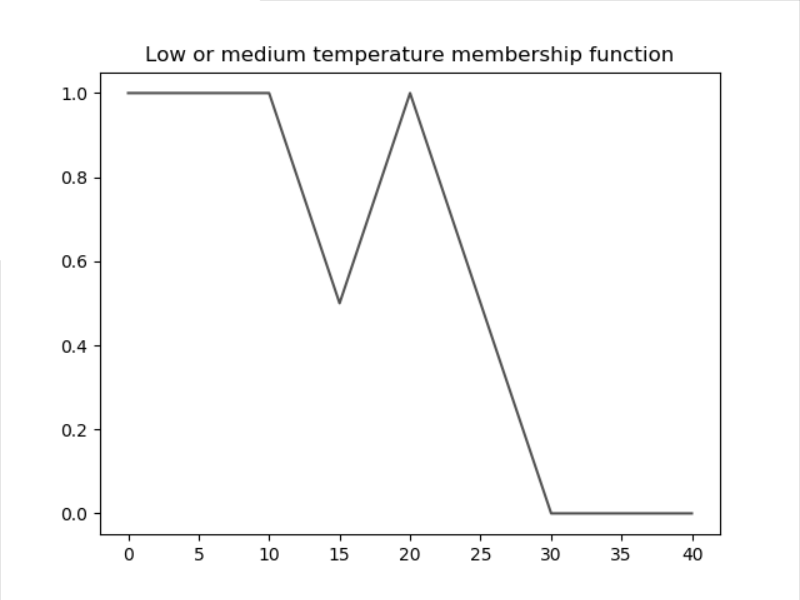
\includegraphics[width=300px]{low_or_medium}
\end{center}

\section*{2. Opérateurs de la logique floue}

J'ai souhaité créer une fonction générique qui calculerait pour n'importe quel ensemble d'opérations logiques les résultats de leurs combinaisons. Cette fonction prend en entrée deux choses :\\
\begin{itemize}
\item Un arbre avec pour chaque feuille une fonction d'appartenance et à chaque autre nœud une d'opération logique à appliquer sur les enfants de ce nœud.
\item Des valeurs qui seront données à chaque fonction d'appartenance pour calculer toutes les opérations sur l'ensemble des valeurs.
\end{itemize}
Reprenons le cas de température basse ou moyenne de l'exercie 1.a. On souhaite calculer les degrés d'appartenance pour la fonction basse et la fonction moyenne, puis appeler \textit{fuzzy\_or} dessus et cela pour chaque valeur. Les valeurs ici sont les valeurs de l'axe des abscisses. On les appelle \textit{x\_data}. On écrit l'arbre d'opération logique dans une liste \textit{low\_or\_medium\_temp}. Cela donne :
\begin{minted}{python}
x_data = np.arange(xMin, xMax, xStep)
low_or_medium_temp = [
    fuzzy_or,
    [low_temp],
    [medium_temp]
]
\end{minted}

Ces paramètres sont alors donnés à ma fonction qui retourne l'ensemble des résultats calculés pour chaque valeur d'entrée.
\begin{minted}{python}
y_data = fuzzy_combine(low_or_medium_temp, x_data)
\end{minted}

Regardons maintenant cette fonction. Il s'agit d'une fonction récursive, qui à chaque récursion calcule le résultat de l'opération logique au nœud de l'arbe à partir du ou des enfants de ce nœud.
Lorsqu'on est sur une feuille de l'arbre, il faut simplement retourner le degré d'appartenance pour chaque valeur.
Lorsqu'on est sur un autre nœud, on applique la fonction logique sur les 1 ou 2 enfants en appelant récursivement \textit{fuzzy\_combine}.
\begin{minted}{python}
def fuzzy_combine(functions, values):
    if len(functions) == 1:
        return list(map(functions[0], values))

    if len(functions) == 2:
        return list(map(functions[0], fuzzy_combine(functions[1], values)))

    if len(functions) == 3:
        return list(map(functions[0], fuzzy_combine(functions[1], values), fuzzy_combine(functions[2], values)))
\end{minted}
\todo{Faire rentrer le code dans le cadre, c'est truncate là}

On peut vérifier que cela marche sur des arbres logiques plus complexes. Par exemple NOT(basse AND élevée) devrait nous retourner 1 pour toutes les valeurs car les fonctions d'appartenance basse et élevée ne s'intersectent pas, et le NOT de 0 est 1.
\begin{minted}{python}
x_data = np.arange(xMin, xMax, xStep)
not_low_and_high_temp = [
    fuzzy_not,
    [
        fuzzy_and,
        [low_temp],
        [high_temp]
    ]
]
y_data = fuzzy_combine(not_low_and_high_temp, x_data)
\end{minted}
\begin{center}
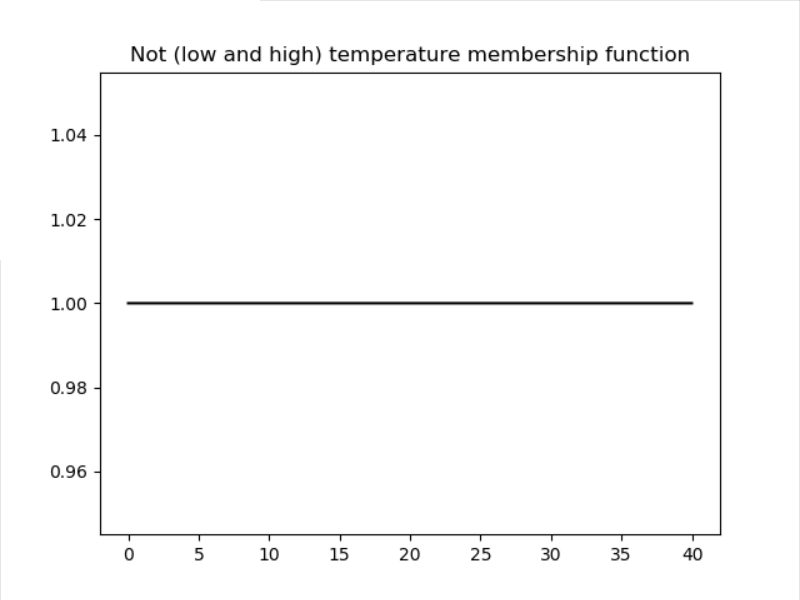
\includegraphics[width=300px]{fuzzy_combine}
\end{center}

\end{document}